\begin{figure}
\renewcommand*{\arraystretch}{0.75}
\setlength{\arraycolsep}{3pt}
\centering
\begin{tikzpicture}
  \node (H) {
    \begin{tikzpicture}
      \node[inner sep=0pt] (gate) at (0,0) {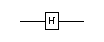
\includegraphics[scale=2]{Figures/circuits/H}};
      \node[below=-2mm of gate] (matrix) {\small\(H = \frac{1}{\sqrt{2}}\){\footnotesize \(\begin{pmatrix} 1 & 1 \\ 1 & -1 \end{pmatrix}\)}};
    \end{tikzpicture}
  };
  \node [right=-4mm of H] (X) {
    \begin{tikzpicture}
      \node[inner sep=0pt] (gate) at (0,0) {\includegraphics[scale=2]{Figures/circuits/X}};
      \node[below=-2mm of gate] (matrix) {\small\(X =\){\footnotesize \(\begin{pmatrix} 0 & 1 \\ 1 & 0 \end{pmatrix}\)}};
    \end{tikzpicture}
  };
  \node [right=-4mm of X] (Y) {
    \begin{tikzpicture}
      \node[inner sep=0pt] (gate) at (0,0) {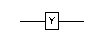
\includegraphics[scale=2]{Figures/circuits/Y}};
      \node[below=-2mm of gate] (matrix) {\small\(Y =\){\footnotesize \(\begin{pmatrix} 0 & -i \\ i & 0 \end{pmatrix}\)}};
    \end{tikzpicture}
  };
  \node [right=-4mm of Y] (Z) {
    \begin{tikzpicture}
      \node[inner sep=0pt] (gate) at (0,0) {\includegraphics[scale=2]{Figures/circuits/Z}};
      \node[below=-2mm of gate] (matrix) {\small\(Z = \){\footnotesize \(\begin{pmatrix} 1 & 0 \\ 0 & -1 \end{pmatrix}\)}};
    \end{tikzpicture}
  };
  \node [below=0mm of H] (S) {
    \begin{tikzpicture}
      \node[inner sep=0pt] (gate) at (0,0) {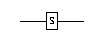
\includegraphics[scale=2]{Figures/circuits/S}};
      \node[below=-2mm of gate] (matrix) {\small\(S =\){\footnotesize \(\begin{pmatrix} 1 & 0 \\ 0 & i \end{pmatrix}\)}};
    \end{tikzpicture}
  };
  \node [below=0mm of X] (T) {
    \begin{tikzpicture}
      \node[inner sep=0pt] (gate) at (0,0) {\includegraphics[scale=2]{Figures/circuits/T}};
      \node[below=-2mm of gate] (matrix) {\small\(T =\){\footnotesize \(\begin{pmatrix} 1 & 0 \\ 0 & e^{i\frac{\pi}{4}} \end{pmatrix}\)}};
    \end{tikzpicture}
  };
  \node [right=0mm of T] (CNOT) {
    \begin{tikzpicture}
      \node[inner sep=0pt] (gate) at (0,0) {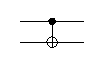
\includegraphics[scale=2]{Figures/circuits/CNOT}};
      \node[left=-5mm of gate] (matrix) {\small\(CNOT = \){\footnotesize \(\begin{pmatrix} 1 & 0 & 0 & 0 \\ 0 & 1 & 0 & 0 \\ 0 & 0 & 0 & 1 \\ 0 & 0 & 1 & 0 \end{pmatrix}\)}};
    \end{tikzpicture}
  };  
\end{tikzpicture}
\caption{The Clifford+T gate set. Both their matrix and circuit representation are given.}
\label{fig:clifford}
\end{figure}